\begin{figure}[H]
    \centering
    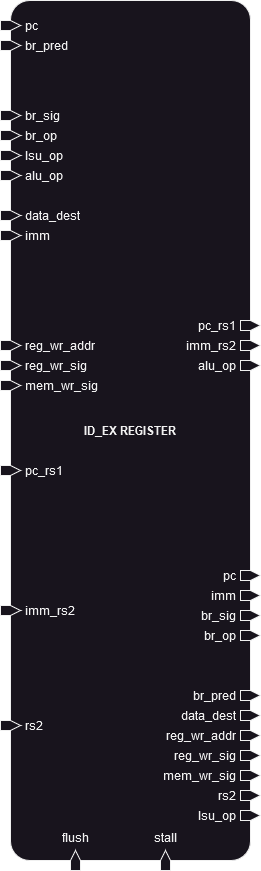
\includegraphics[width=0.35\textwidth]{design/pipelined/pipeline/images/pipeline.png}
    \caption{ID-EX Pipeline register example}
    \label{fig:pipeline}
\end{figure}

I will not explain the 4 different pipeline register stages in detail, and I will mainly describe as an example the 
pipeline between the ID Stage and the Ex Stage. The role of a pipeline register is to store the data that will be
passed to the next stage at each clock cycle such that you can increase throughput by increasing the clock frequency since 
you've divided the overall work in smaller chunks so you can do it in less time (theoretically).
What is also interesting here is the $stall$ and $flush$ signals. The first one is used to stop updating the pipeline when 
a data dependency is encountered. The second one is used when the branch predictor did a bad guess. In this case we need to 
flush the register that has incorrect instructions stored in them and instead just fill them with something similar to a NOP 
instruction.